\ifdefined\iscombined
	\quiz{Quiz 3}
\else
\documentclass{article}
\usepackage{xparse}
\usepackage{tabularx}
\usepackage{changepage}
\usepackage{listings}
\usepackage{amsthm}
\usepackage{comment}
\usepackage{amsmath}
\usepackage{braket}
\usepackage{amsfonts}
\usepackage{amssymb}
\usepackage{sectsty}
\usepackage{hyperref}
\usepackage{fancyhdr}
\usepackage[top=1in,bottom=1in,left=1in,right=1in]{geometry}
\usepackage{float}
\usepackage{graphicx}
\usepackage{mathtools}
\usepackage{tikz}
\usepackage{enumitem}
\usetikzlibrary{arrows, arrows.meta}

\date{
	\vspace{-.75em}
	{\large \today}
}

\title{
	\vspace*{-1.5em}
	{\Huge Quiz 3} \\
	\vspace{-1em}
	\rule{\textwidth/2}{.01em} \\
	\vspace{-.75em}
}

\author{
	{\large Matthew Farah}
}

\hypersetup{
	colorlinks=true,
	linkcolor=blue,
	filecolor=magenta,
	urlcolor=blue,
	citecolor=blue,
	anchorcolor=blue
}

\fancyhead{}
\fancyhead[L]{\today}
\fancyhead[R]{Quiz 3}

\setlength{\parindent}{0cm}

\tikzset{vertex/.style = {shape = circle, draw, minimum size = 2em}}
\tikzset{edge/.style = {-,> = latex'}}

\newenvironment{solution}{
	\vspace{.5em}
	\par
	\begin{adjustwidth}{1.5em}{}
	\textbf{{Solution:}}
	\par
	\vspace{.5em}
}{
	\vspace{1em}
	\end{adjustwidth}
	\setcounter{step}{0}
}

\makeatother
\makeatletter

\newcounter{step}
\renewcommand{\thestep}{\Roman{step}}

\newenvironment{step}{
	\refstepcounter{step}
	\setcounter{substep}{0}
	\vspace{1em}\par\noindent
	\ignorespaces\noindent\textbf{(\thestep)}
	\ignorespaces
}{
	\par
	\vspace{1.5em}
}

\newcounter{substep}
\renewcommand{\thesubstep}{\alph{substep}}

\newenvironment{substep}{
	\refstepcounter{substep}
	\vspace{1em}\par\noindent
	\ignorespaces\noindent\textbf{(\thesubstep)}
	\ignorespaces
}{
	\par
	\vspace{1.5em}
}


\newcounter{problem}
\renewcommand{\theproblem}{\arabic{problem}}

\newenvironment{problem}[1][]{
	\newpage
	\refstepcounter{problem}
	\setcounter{subproblem}{0}
	\vspace{.5em}\par\noindent
	\begin{adjustwidth}{1.5em}{}
	\noindent\textbf{Problem \theproblem: }\noindent\textit{#1}
	\par
	\phantomsection
	\addcontentsline{toc}{section}{\protect{\large{Problem \theproblem}}}
}{
	\vspace{.5em}
	\end{adjustwidth}
}

\newcounter{subproblem}
\renewcommand{\thesubproblem}{\alph{subproblem}}

\newenvironment{subproblem}{
	\setcounter{step}{0}
	\refstepcounter{subproblem}
	\phantomsection
	\addcontentsline{toc}{subsection}{\protect{\large{(\thesubproblem)}}}
	\begin{adjustwidth}{1.5em}{}
	\noindent{\textbf{(\thesubproblem) }}\ignorespaces
}{
	\par
	\vspace{.5em}
	\end{adjustwidth}
}

\newcounter{lemma}
\renewcommand{\thelemma}{\arabic{lemma}}

\newenvironment{lemma}[1][]{
	\refstepcounter{lemma}
	\vspace{1em}\par\noindent
	\noindent\textbf{Lemma ({#1}): }\noindent\ignorespaces
}{
	\vspace{.5em}
}

\newcounter{proposition}
\renewcommand{\theproposition}{\arabic{proposition}}

\newenvironment{proposition}{
	\refstepcounter{proposition}
	\vspace{1em}\par\noindent
	\noindent\textbf{Proposition: }\noindent\ignorespaces
}{
	\vspace{.5em}
}

\newcommand{\supp}[1]{\text{supp}({#1})}
\newcommand{\ord}[1]{\text{ord}\left({#1}\right)}
\newcommand{\gen}[1]{\left\langle {#1} \right\rangle}
\newcommand{\lcm}[2]{\text{lcm}({#1}, {#2})}
\newcommand{\dprod}[2]{\mathbb{Z}_{#1} \times \mathbb{Z}_{#2}}

\renewcommand{\mod}[1]{\ (\text{mod} \; {#1})}

\sectionfont{\fontsize{12}{12}\bfseries}
\subsectionfont{\fontsize{10}{12}\normalfont}
\subsubsectionfont{\fontsize{10}{12}\normalfont}

\begin{document}

\maketitle
\pagestyle{fancy}

\newcolumntype{Y}{>{\centering\arraybackslash}X}

\tableofcontents

\fi

\newpage

Please note the quiz is based on the following topics:
\begin{itemize}
	\item Conjugation.
	\item Normal Subgroups.
\end{itemize}

% NOTE: Problem 1
\begin{problem}
	In the group $D_{4}$, let $r= (1234)$ be a clockwise rotation, and let $s = (12)(34)$ be a reflection. Which of the following elements are equal to $sr$?
\end{problem}

%NOTE: Problem 1 (a)
\begin{subproblem}
	$rs$.
\end{subproblem}

\begin{solution}
	$rs$ does not equal $sr$. \\

	For this and the following questions, we will use the fact that:

	\begin{align*}
		sr &= (12)(34)(1234) \\
		&= (24) \\
	\end{align*}

	Which graphically looks like the following adjacency-preserving permutation of the vertices of a square:

	\vspace{2em}
	
	\begin{minipage}{0.40\textwidth}
		\begin{center}
			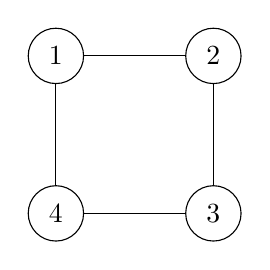
\begin{tikzpicture}
				\node[vertex] (a) at (0, 2) {$1$};
				\node[vertex] (b) at (2, 2) {$2$};
				\node[vertex] (c) at (2, 0) {$3$};
				\node[vertex] (d) at (0, 0) {$4$};
	
				\draw[edge] (a) to (b);
				\draw[edge] (b) to (c);
				\draw[edge] (c) to (d);
				\draw[edge] (d) to (a);
			\end{tikzpicture}
		\end{center}
	\end{minipage}
	\begin{minipage}{0.04\textwidth}
		\begin{center}
			\begin{tikzpicture}
				\draw[-{Stealth[length=1.25mm, width=1mm]}, line width=0.01pt] (0,0) -- (2.5,0)
				node[midway, above=2pt] {$sr$};
			\end{tikzpicture}
		\end{center}
	\end{minipage}
	\begin{minipage}{0.56\textwidth}
		\begin{center}
			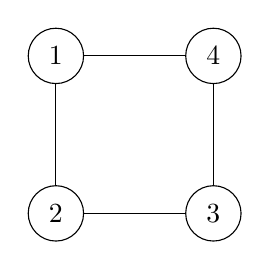
\begin{tikzpicture}
				\node[vertex] (a) at (0, 2) {$1$};
				\node[vertex] (b) at (2, 2) {$4$};
				\node[vertex] (c) at (2, 0) {$3$};
				\node[vertex] (d) at (0, 0) {$2$};
	
				\draw[edge] (a) to (b);
				\draw[edge] (b) to (c);
				\draw[edge] (c) to (d);
				\draw[edge] (d) to (a);
			\end{tikzpicture}
		\end{center}
	\end{minipage}

	\vspace{2em}

	to determine whether or not the given permutations are equivalent to $sr$. In this case, since:

	\begin{align*}
		rs &= (1234)(12)(34) \\
		&= (13) \\
	\end{align*}

	Which can be graphically represented by the transformation:

	\vspace{2em}
	
	\begin{minipage}{0.40\textwidth}
		\begin{center}
			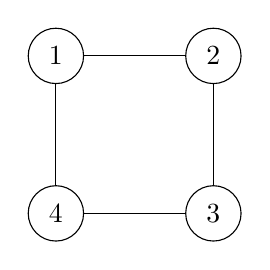
\begin{tikzpicture}
				\node[vertex] (a) at (0, 2) {$1$};
				\node[vertex] (b) at (2, 2) {$2$};
				\node[vertex] (c) at (2, 0) {$3$};
				\node[vertex] (d) at (0, 0) {$4$};
	
				\draw[edge] (a) to (b);
				\draw[edge] (b) to (c);
				\draw[edge] (c) to (d);
				\draw[edge] (d) to (a);
			\end{tikzpicture}
		\end{center}
	\end{minipage}
	\begin{minipage}{0.04\textwidth}
		\begin{center}
			\begin{tikzpicture}
				\draw[-{Stealth[length=1.25mm, width=1mm]}, line width=0.01pt] (0,0) -- (2.5,0)
				node[midway, above=2pt] {$rs$};
			\end{tikzpicture}
		\end{center}
	\end{minipage}
	\begin{minipage}{0.56\textwidth}
		\begin{center}
			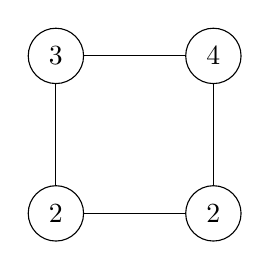
\begin{tikzpicture}
				\node[vertex] (a) at (0, 2) {$3$};
				\node[vertex] (b) at (2, 2) {$4$};
				\node[vertex] (c) at (2, 0) {$2$};
				\node[vertex] (d) at (0, 0) {$2$};
	
				\draw[edge] (a) to (b);
				\draw[edge] (b) to (c);
				\draw[edge] (c) to (d);
				\draw[edge] (d) to (a);
			\end{tikzpicture}
		\end{center}
	\end{minipage}

	\vspace{2em}

	It is clear that $rs$ and $sr$ are different permutations, and thus, are unequal.
\end{solution}

%NOTE: Problem 1 (b)
\begin{subproblem}
	$r^{2}s$.
\end{subproblem}

\begin{solution}
	$r^{2}s$ doesn't equal $sr$ as well. To see why, we can leverage the fact that $rs = (13)$ (which we determined in part \textbf{(a)}) to conclude that:

	\begin{align*}
		r^{2}s &= r(rs) \\
		&= (1234)(13) \\
		&= (14)(23) \\
	\end{align*}

	Which visually looks like this:

	\vspace{2em}
	
	\begin{minipage}{0.40\textwidth}
		\begin{center}
			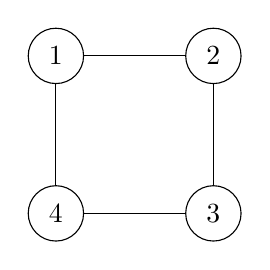
\begin{tikzpicture}
				\node[vertex] (a) at (0, 2) {$1$};
				\node[vertex] (b) at (2, 2) {$2$};
				\node[vertex] (c) at (2, 0) {$3$};
				\node[vertex] (d) at (0, 0) {$4$};
	
				\draw[edge] (a) to (b);
				\draw[edge] (b) to (c);
				\draw[edge] (c) to (d);
				\draw[edge] (d) to (a);
			\end{tikzpicture}
		\end{center}
	\end{minipage}
	\begin{minipage}{0.04\textwidth}
		\begin{center}
			\begin{tikzpicture}
				\draw[-{Stealth[length=1.25mm, width=1mm]}, line width=0.01pt] (0,0) -- (2.5,0)
				node[midway, above=2pt] {$r^{2}s$};
			\end{tikzpicture}
		\end{center}
	\end{minipage}
	\begin{minipage}{0.56\textwidth}
		\begin{center}
			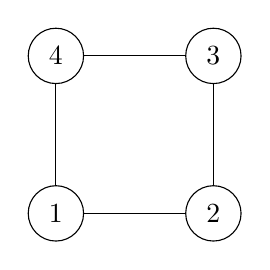
\begin{tikzpicture}
				\node[vertex] (a) at (0, 2) {$4$};
				\node[vertex] (b) at (2, 2) {$3$};
				\node[vertex] (c) at (2, 0) {$2$};
				\node[vertex] (d) at (0, 0) {$1$};
	
				\draw[edge] (a) to (b);
				\draw[edge] (b) to (c);
				\draw[edge] (c) to (d);
				\draw[edge] (d) to (a);
			\end{tikzpicture}
		\end{center}
	\end{minipage}

	\vspace{2em}

	And since this is clearly a different permutation than $sr$, $r^{2}s \neq sr$.
\end{solution}

%NOTE: Problem 1 (c)
\begin{subproblem}
	$r^{3}s$.
\end{subproblem}

\begin{solution}
	$r^{3}s$ actually does equal $sr$!

	Proceeding as we did before, since:

	\begin{align*}
		r^{3}s &= r(r^{2}s) \\
		&= (1234)(14)(23) \\
		&= (24) \\
	\end{align*}

	Which looks like:

	\vspace{2em}
	
	\begin{minipage}{0.40\textwidth}
		\begin{center}
			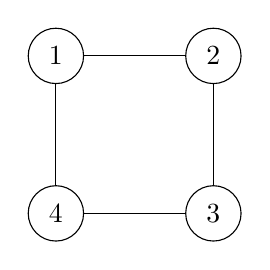
\begin{tikzpicture}
				\node[vertex] (a) at (0, 2) {$1$};
				\node[vertex] (b) at (2, 2) {$2$};
				\node[vertex] (c) at (2, 0) {$3$};
				\node[vertex] (d) at (0, 0) {$4$};
	
				\draw[edge] (a) to (b);
				\draw[edge] (b) to (c);
				\draw[edge] (c) to (d);
				\draw[edge] (d) to (a);
			\end{tikzpicture}
		\end{center}
	\end{minipage}
	\begin{minipage}{0.04\textwidth}
		\begin{center}
			\begin{tikzpicture}
				\draw[-{Stealth[length=1.25mm, width=1mm]}, line width=0.01pt] (0,0) -- (2.5,0)
				node[midway, above=2pt] {$r^{3}s$};
			\end{tikzpicture}
		\end{center}
	\end{minipage}
	\begin{minipage}{0.56\textwidth}
		\begin{center}
			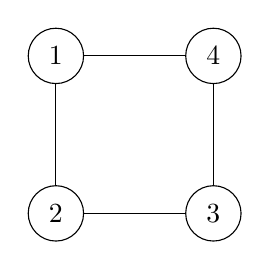
\begin{tikzpicture}
				\node[vertex] (a) at (0, 2) {$1$};
				\node[vertex] (b) at (2, 2) {$4$};
				\node[vertex] (c) at (2, 0) {$3$};
				\node[vertex] (d) at (0, 0) {$2$};
	
				\draw[edge] (a) to (b);
				\draw[edge] (b) to (c);
				\draw[edge] (c) to (d);
				\draw[edge] (d) to (a);
			\end{tikzpicture}
		\end{center}
	\end{minipage}

	\vspace{2em}

	We can see that $r^{3}s$ is indeed the same permutation as $sr$, and so $r^{3}s = sr$.
\end{solution}

%NOTE: Problem 1 (d)
\begin{subproblem}
	$r^{4}s$.
\end{subproblem}

\begin{solution}
	$r^{4}s$ doesn't equal $sr$. \\

	This is because:

	\begin{align*}
		r^{4}s &= r(r^{3}s) \\
		&= (1234)(24) \\
		&= (12)(34) \\
	\end{align*}

	Or, graphically:

	\vspace{2em}
	
	\begin{minipage}{0.40\textwidth}
		\begin{center}
			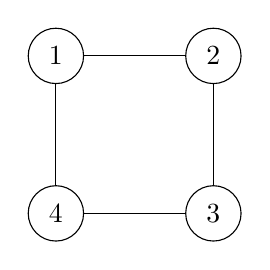
\begin{tikzpicture}
				\node[vertex] (a) at (0, 2) {$1$};
				\node[vertex] (b) at (2, 2) {$2$};
				\node[vertex] (c) at (2, 0) {$3$};
				\node[vertex] (d) at (0, 0) {$4$};
	
				\draw[edge] (a) to (b);
				\draw[edge] (b) to (c);
				\draw[edge] (c) to (d);
				\draw[edge] (d) to (a);
			\end{tikzpicture}
		\end{center}
	\end{minipage}
	\begin{minipage}{0.04\textwidth}
		\begin{center}
			\begin{tikzpicture}
				\draw[-{Stealth[length=1.25mm, width=1mm]}, line width=0.01pt] (0,0) -- (2.5,0)
				node[midway, above=2pt] {$r^{4}s$};
			\end{tikzpicture}
		\end{center}
	\end{minipage}
	\begin{minipage}{0.56\textwidth}
		\begin{center}
			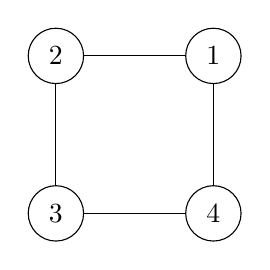
\begin{tikzpicture}
				\node[vertex] (a) at (0, 2) {$2$};
				\node[vertex] (b) at (2, 2) {$1$};
				\node[vertex] (c) at (2, 0) {$4$};
				\node[vertex] (d) at (0, 0) {$3$};
	
				\draw[edge] (a) to (b);
				\draw[edge] (b) to (c);
				\draw[edge] (c) to (d);
				\draw[edge] (d) to (a);
			\end{tikzpicture}
		\end{center}
	\end{minipage}

	\vspace{2em}

	Thus, $r^{4}s$ and $sr$ are clearly different permutations and so $r^{4}s \neq sr$.
\end{solution}

%NOTE: Problem 2
\begin{problem}
	Let $G$ be a group, and let $a \in G$. What notations represent the conjugacy class of $a$?
\end{problem}

\begin{solution}
	$a^{G}$ and $[a]$ are both ways of denoting the conjugacy class of $a$. Note that $a^{G}$ is perhaps a little more descriptive than $[a]$, since it explicitly states which group it is a conjugacy class of.
\end{solution}

%NOTE: Problem 3
\begin{problem}
	Let $G$ be a group and let $a, b \in G$. What is the definition of $a^{b}$?
\end{problem}

\begin{solution}
	$a^{b}$ is defined by:

	\begin{align*}
		a^{b} &= b^{-1}ab
	\end{align*}
\end{solution}

%NOTE: Problem 4
\begin{problem}
	If $\sigma = (153)(24)$ and $g = (5314)$, then what does $\sigma^{g}$ equal?
\end{problem}

\begin{solution}
	By the definition of $\sigma^{g}$ given as the solution to the problem just above, we know that:

	\begin{align*}
		\sigma^{g} &= g^{-1}\sigma{g} &&\text{(By definition of conjugation)} \\
		&= (5314)^{-1}(153)(24)(5314) &&\text{(Substituting)} \\
	\end{align*}

	So, to compute $\sigma^{g}$, we'll need to find $g^{-1}$! This is thankfully not very difficult to do. Although I won't prove it (:P), it is generally true that the inverse of any permutation of the form $(abc\ldots{z})$ is just $(zxy\ldots{a})$, and so $g^{-1} = (4135)$. \\

	So carrying out our earlier computation, we have that:

	\begin{align*}
		\sigma^{g} &= (5314)^{-1}(153)(24)(5314) &&\text{(From earlier equation)} \\
		&= (4135)(153)(24)(5314) &&\text{(Since $(5314)^{-1} = (4135)$)} \\
		&= (4135)(12435) &&\text{(Simplifying)} \\
		&= (12)(345) &&\text{(Simplifying)} \\
	\end{align*}

	Thus, $\sigma^{g} = (12)(345)$.
\end{solution}

%NOTE: Problem 5
\begin{problem}
	Find all elements $g \in S_{3}$ such that $g^{-1}(123)g = (132)$.
\end{problem}

\begin{solution}
	We know that $S_{3} = \set{(), (12), (23), (13), (123), (132)}$ so, together with the quick and easy method for finding the inverse of a permutation I mentioned in the solution to the problem above, we can brute force all possible $g \in S_{3}$ to find that:

	\begin{step}
		When $g = ()$:
	\end{step}

	\begin{align*}
		g^{-1}(123)g &= ()(123)() \\
		&= ()(123) \\
		&= (123) \\
	\end{align*}

	\begin{step}
		When $g = (12)$:
	\end{step}

	\begin{align*}
		g^{-1}(123)g &= (21)(123)(12) \\
		&= (21)(13) \\
		&= \boxed{(132)} \\
	\end{align*}

	\begin{step}
		When $g = (23)$:
	\end{step}

	\begin{align*}
		g^{-1}(123)g &= (32)(123)(23) \\
		&= (32)(12) \\
		&= \boxed{(132)} \\
	\end{align*}

	\begin{step}
		When $g = (13)$:
	\end{step}

	\begin{align*}
		g^{-1}(123)g &= (31)(123)(13) \\
		&= (31)(23) \\
		&= \boxed{(132)}
	\end{align*}

	\begin{step}
		When $g = (123)$:
	\end{step}

	\begin{align*}
		g^{-1}(123)g &= (321)(123)(123) \\
		&= (321)(132) \\
		&= (123) \\
	\end{align*}

	\begin{step}
		When $g = (132)$:
	\end{step}

	\begin{align*}
		g^{-1}(123)g &= (231)(123)(132) \\
		&= (231)() \\
		&= (231) \\
		&= (123) \\
	\end{align*}

	Thus, the set of all $g$ in $S_{3}$ satisfying $g^{-1}(123)g = (132)$ is $\set{(12), (23), (13)}$.
\end{solution}

%NOTE: Problem 6
\begin{problem}
	How many elements do the following conjugacy classes contain?
\end{problem}

%NOTE: Problem 6 (a)
\begin{subproblem}
	$[(123)]$ in $S_{4}$.
\end{subproblem}

\begin{solution}
	$[(123)]$ in $S^{4}$ has 8 elements. \\

	By Theorem 5.3, we know that $(123)$ is conjugate to another permutation, $\tau \in S_{4}$, if and only if $(123)$ and $\tau$ have the same cycle type. \\

	The cycle type of $(123)$ in $S_{4}$ is $(3, 1)$ and so all permutations in $S_{4}$ conjugate to $(123)$ must likewise have a cycle type of $(3, 1)$. Therefore, all permutations in $S_{4}$ conjugate to $(123)$ are expressible as $(abc)$, where $a, b, c \in \set{1, 2, 3, 4}$ and $a, b$, and $c$ are all pairwise distinct. \\

	Clearly then, there are $4! = 24$ possible such permutations in $S_{4}$, since:
	\begin{itemize}
		\item There are $4$ possible choices for $a$.
		\item 3 choices for $b$ so as to not conflict with $a$.
		\item 2 for $c$ to avoid conflicting with both $a$ and $b$.
		\item Only one choice as to which element the permutation leave fixed, after $a, b$, and $c$ have all been chosen. \\
	\end{itemize}

	However, recall that the permutations $(abc)$, $(bca)$, and $(cab)$ are all equivalent, meaning 24 over counts the number of distinct such permutations in $S_{4}$ by a factor of 3. Thus, there are actually $\frac{24}{3} = 8$ permutations with a cycle type of $(3, 1)$ in $S_{4}$. \\

	Thus, since there are exactly 8 permutations in $S_{4}$ with the same cycle type as $(123)$, there are also exactly 8 elements in the conjugacy class of $(123)$.
\end{solution}

%FIX: Problem 6 (b)
\begin{subproblem}
	$[(123)]$ in $A_{4}$.
\end{subproblem}

\begin{solution}

\end{solution}

%NOTE: Problem 6 (c)
\begin{subproblem}
	$[5]$ in $\mathbb{Z}^{\times}_{6}$.
\end{subproblem}

\begin{solution}
	$[5]$ in $\mathbb{Z}^{\times}_{6}$ has 1 element. \\

	$\mathbb{Z}^{\times}_{6}$ is a relatively small group, so we will find the size of $[5]$ in $\mathbb{Z}^{\times}_{6}$ by brute force. By Proposition 1.7, we know that because:

	\vspace{2em}

	\begin{tabularx}{\linewidth}{Y Y}
		$\gcd(0, 6) = 6$ & $\gcd(3, 6) = 3$ \\
		$\boxed{\gcd(1, 6) = 1}$ & $\gcd(4, 6) = 2$ \\
		$\gcd(2, 6) = 2$ & $\boxed{\gcd(5, 6) = 1}$ \\
	\end{tabularx}

	\vspace{2em}

	1 and 5 are the only units modulo 6. Thus, $\mathbb{Z}^{\times}_{6} = \set{1, 5}$. Now, since:

	\begin{align*}
		5^{1} &\equiv (1)^{-1}(5)(1) \mod{6} \\
		&\equiv (1)(5)(1) \mod{6} \\
		&\equiv (1)(5) \mod{6} \\
		&\equiv 5 \mod{6} \\
		&\equiv 5 \\
	\end{align*}

	and:

	\begin{align*}
		5^{5} &\equiv (5)^{-1}(5)(5) \mod{6} \\
		&\equiv (5)(5)(5) \mod{6} \\
		&\equiv (5)(25) \mod{6} \\
		&\equiv 125 \mod{6} \\
		&\equiv 5 \\
	\end{align*}

	We therefore have that the conjugacy class of $5$ in $\mathbb{Z}^{\times}_{6}$ is just the set containing 5. Thus, since $[5] = \set{5}$, $[5]$ contains only one element.
\end{solution}

%NOTE: Problem 7
\begin{problem}
	How many conjugacy classes are there in $S_{5}$.
\end{problem}

\begin{solution}
	There are 7 conjugacy classes in $S_{5}$. \\

	By Theorem 5.3 and the fact that conjugacy classes form equivalence partitions over their domain, we know there must be as many conjugacy classes in $S_{5}$ as there are distinct cycle types in $S_{5}$. \\

	Since there are 7 distinct cycle types in $S_{5}$, given by the set $\set{(1, 1, 1, 1, 1), (2, 1, 1, 1), (2, 2, 1), (3, 1, 1), (3, 2), (4, 1), (5)}$, (derived from the integer partitions of 5), there must therefore be 7 conjugacy classes in $S_{5}$, as argued earlier.
\end{solution}

%NOTE: Problem 8
\begin{problem}
	Which of the following subgroups are normal subgroups of $G = GL_{2}(\mathbb{Z}_{2})$?
\end{problem}

%NOTE: Problem 8 (a)
\begin{subproblem}
	$H = \left\{
		\begin{pmatrix}
			1 & 0 \\
			0 & 1
		\end{pmatrix},
		\begin{pmatrix}
			0 & 1 \\
			1 & 1
		\end{pmatrix},
		\begin{pmatrix}
			1 & 1 \\
			1 & 0
		\end{pmatrix}
	\right\}$
\end{subproblem}

\begin{solution}
	$H$ is a normal subgroup of $G$. \\

	To see why, recall that for $H$ to be a normal subgroup of $G$, it must be closed under conjugation, meaning that for all $g \in G$ and $h \in H$, $h^{g} \in H$. Since I couldn't really think of a better way, our approach will be to compute $h^{g}$ for all possible $h$ and $g$, but cleverly take shortcuts where possible to cut down on the number of required calculations. \\

	For one, since $h^{g} = g^{-1}hg$, it'd be convenient to have an easy formula for $g^{-1}$, given $g$, that we can use to plug and chug with. It is for that reason that I will quickly sidetrack to prove that for any $g \in G$ of the form:

	\begin{align*}
		g &= \begin{pmatrix}
			a & b \\
			c & d
		\end{pmatrix}
	\end{align*}
	
	$g^{-1} \in G$ is given by:

	\begin{align*}
		g^{-1} &= \begin{pmatrix}
			d & b \\
			c & a
		\end{pmatrix}
	\end{align*}
	
	To understand how this is the case, all that's required is to understand two things:
	\begin{enumerate}
		\item For any $x \in \mathbb{Z}_{2}, 2x = 0$.
		\begin{itemize}
			\item This is because if $x = 0$, then $2x = (2)(0) \equiv 0$, and if $x = 1$, then $(2)(1) = 2 = 0 \mod{2}$.
		\end{itemize}
		\item $ad + bc = 1$.
		\begin{itemize}
			\item This is because exactly one of $ad$ or $bc$ can be 1, and the other must be 0.
			\begin{itemize}
				\item Since $\det(g) = ad - bc \neq 0$, by definition of $g$ belonging to $GL_{2}(\mathbb{Z}_{2})$. \\
			\end{itemize}
		\end{itemize}
	\end{enumerate}

	And so, we have that:

	\begin{align*}
		\boxed{\begin{pmatrix}
			d & b \\
			c & a
		\end{pmatrix}
		\begin{pmatrix}
			a & b \\
			c & d
		\end{pmatrix}}
		&= \begin{pmatrix}
			ad + cb & db + bd \\
			ca + ac & cb + ad
		\end{pmatrix}
		&&\text{(Simplifying)} \\\\
		&= \begin{pmatrix}
			ad + bc & 2bd \\
			2ac & ad + bc
		\end{pmatrix}
		&&\text{(Simplifying)} \\\\
		&= \begin{pmatrix}
			ad + bc & 0 \\
			0 & ad + bc
		\end{pmatrix}
		&&\text{(Since $2x = 0$ for all $x \in \mathbb{Z}_{2}$)} \\\\
		&= \boxed{\begin{pmatrix}
			1 & 0 \\
			0 & 1
		\end{pmatrix}}
		&&\text{(Since $ad + bc = 1$)} \\\\
		&= \begin{pmatrix}
			bc + ad & 0 \\
			0 & bc + ad
		\end{pmatrix}
		&&\text{(Since $bc + ad = 1$)} \\\\
		&= \begin{pmatrix}
			bc + ad & 2ab \\
			2cd & bc + ad
		\end{pmatrix}
		&&\text{(Since $2x = 0$ for all $x \in \mathbb{Z}_{2}$)} \\\\
		&= \boxed{\begin{pmatrix}
			a & b \\
			c & d
		\end{pmatrix}
		\begin{pmatrix}
			d & b \\
			c & a
		\end{pmatrix}} \\\\
	\end{align*}

	And thus, $g^{-1} = \begin{pmatrix} d & b \\ c & a \end{pmatrix}$. So now that we know how to compute $g^{-1}hg$, we need only consider 3 possible cases, recalling that we need only check that $h$ is closed under conjuigation by $\begin{pmatrix} 0 & 1 \\ 1 & 0 \end{pmatrix}, \begin{pmatrix} 1 & 0 \\ 1 & 1 \end{pmatrix}$, and $\begin{pmatrix} 1 & 1 \\ 0 & 1 \end{pmatrix}$, since all other matrices in $GL_{2}(\mathbb{Z}_{2})$ belong to $H$, which is given to be a group.

	\begin{step}
		$h = \begin{pmatrix} 1 & 0 \\ 0 & 1 \end{pmatrix}$.
	\end{step}

	If $h = \begin{pmatrix} 1 & 0 \\ 0 & 1 \end{pmatrix}$, then we wouldn't even need to consider the different choices of $g$ to see that:

	\begin{align*}
		h^{g} &= g^{-1}
		\begin{pmatrix}
			1 & 0 \\
			0 & 1
		\end{pmatrix}
		g
		&& \text{(By definition of conjugation)} \\\\
		&= g^{-1}g &&\text{(By definition of the identity)} \\\\
		&= \begin{pmatrix}
			1 & 0 \\
			0 & 1
		\end{pmatrix}
		&&\text{(By definition of inverses)} \\\\
	\end{align*}

	And because $\begin{pmatrix} 1 & 0 \\ 0 & 1 \end{pmatrix} \in H, h^{g} \in H$ in this case. (Note that we also could've determined this from the fact the conjugacy class of the identity element is always the set containing just itself).

	\begin{step}
		$h = \begin{pmatrix} 1 & 0 \\ 1 & 1 \end{pmatrix}$.
	\end{step}

	Here, we'll need to consider each possible $g$ individually.

	\begin{substep}
		$g = \begin{pmatrix} 0 & 1 \\ 1 & 0 \end{pmatrix}$.
	\end{substep}

	If $g = \begin{pmatrix} 0 & 1 \\ 1 & 0 \end{pmatrix}$, then $g^{-1} = \begin{pmatrix} 0 & 1 \\ 1 & 0 \end{pmatrix}$, and so we can compute:

	\begin{align*}
		h^{g} &= g^{-1}hg  &&\text{(By definition of conjugation)} \\\\
		&= \begin{pmatrix}
			0 & 1 \\
			1 & 0
		\end{pmatrix}
		\begin{pmatrix}
			0 & 1 \\
			1 & 1
		\end{pmatrix}
		\begin{pmatrix}
			0 & 1 \\
			1 & 0
		\end{pmatrix}
		&&\text{(Substituting)} \\\\
		&= \begin{pmatrix}
			0 & 1 \\
			1 & 0
		\end{pmatrix}
		\begin{pmatrix}
			1 & 0 \\
			1 & 1
		\end{pmatrix}
		&&\text{(Simplifying)} \\\\
		&= \begin{pmatrix}
			1 & 1 \\
			1 & 0
		\end{pmatrix}
		&&\text{(Simplifying)} \\\\
	\end{align*}

	And since $\begin{pmatrix} 1 & 1 \\ 1 & 0 \end{pmatrix} \in H, h^{g} \in H$ in this case.

	\begin{substep}
		$g = \begin{pmatrix} 1 & 0 \\ 1 & 1 \end{pmatrix}$.
	\end{substep}

	If $g = \begin{pmatrix} 1 & 0 \\ 1 & 1 \end{pmatrix}$, then $g^{-1} = \begin{pmatrix} 1 & 0 \\ 1 & 1 \end{pmatrix}$, and so we can compute:

	\begin{align*}
		h^{g} &= g^{-1}hg  &&\text{(By definition of conjugation)} \\\\
		&= \begin{pmatrix}
			1 & 0 \\
			1 & 1
		\end{pmatrix}
		\begin{pmatrix}
			0 & 1 \\
			1 & 1
		\end{pmatrix}
		\begin{pmatrix}
			1 & 0 \\
			1 & 1
		\end{pmatrix}
		&&\text{(Substituting)} \\\\
		&= \begin{pmatrix}
			1 & 0 \\
			1 & 1
		\end{pmatrix}
		\begin{pmatrix}
			1 & 1 \\
			0 & 1
		\end{pmatrix}
		&&\text{(Simplifying)} \\\\
		&= \begin{pmatrix}
			1 & 1 \\
			1 & 0
		\end{pmatrix}
		&&\text{(Simplifying)} \\\\
	\end{align*}

	And since $\begin{pmatrix} 1 & 1 \\ 1 & 0 \end{pmatrix} \in H, h^{g} \in H$ in this case as well.

	\begin{substep}
		$g = \begin{pmatrix} 1 & 1 \\ 0 & 1 \end{pmatrix}$.
	\end{substep}

	If $g = \begin{pmatrix} 1 & 1 \\ 0 & 1 \end{pmatrix}$, then $g^{-1} = \begin{pmatrix} 1 & 1 \\ 0 & 1 \end{pmatrix}$, and so we can compute:

	\begin{align*}
		h^{g} &= g^{-1}hg  &&\text{(By definition of conjugation)} \\\\
		&= \begin{pmatrix}
			1 & 1 \\
			0 & 1
		\end{pmatrix}
		\begin{pmatrix}
			0 & 1 \\
			1 & 1
		\end{pmatrix}
		\begin{pmatrix}
			1 & 1 \\
			0 & 1
		\end{pmatrix}
		&&\text{(Substituting)} \\\\
		&= \begin{pmatrix}
			1 & 1 \\
			0 & 1
		\end{pmatrix}
		\begin{pmatrix}
			0 & 1 \\
			1 & 0
		\end{pmatrix}
		&&\text{(Simplifying)} \\\\
		&= \begin{pmatrix}
			1 & 1 \\
			1 & 0
		\end{pmatrix}
		&&\text{(Simplifying)} \\\\
	\end{align*}

	And since $\begin{pmatrix} 1 & 1 \\ 1 & 0 \end{pmatrix} \in H, h^{g} \in H$ once again.

	Thus, since $h^{g} \in H$ in cases \textbf{(a)}, \textbf{(b)}, and \textbf{(c)}, we have that $h = \begin{pmatrix} 0 & 1 \\ 1 & 1 \end{pmatrix}$ in $H$ is closed under conjugation.

	\begin{step}
		$h = \begin{pmatrix} 1 & 1 \\ 1 & 0 \end{pmatrix}$.
	\end{step}

	We'll once again have to consider each case of $g$ separately.

	\begin{substep}
		$g = \begin{pmatrix} 0 & 1 \\ 1 & 0 \end{pmatrix}$.
	\end{substep}

	When $g = \begin{pmatrix} 0 & 1 \\ 1 & 0 \end{pmatrix}$, then $g^{-1} = \begin{pmatrix} 0 & 1 \\ 1 & 0 \end{pmatrix}$, and so:

	\begin{align*}
		h^{g} &= g^{-1}hg  &&\text{(By definition of conjugation)} \\\\
		&= \begin{pmatrix}
			0 & 1 \\
			1 & 0
		\end{pmatrix}
		\begin{pmatrix}
			1 & 1 \\
			1 & 0
		\end{pmatrix}
		\begin{pmatrix}
			0 & 1 \\
			1 & 0
		\end{pmatrix}
		&&\text{(Substituting)} \\\\
		&= \begin{pmatrix}
			0 & 1 \\
			1 & 0
		\end{pmatrix}
		\begin{pmatrix}
			1 & 1 \\
			0 & 1
		\end{pmatrix}
		&&\text{(Simplifying)} \\\\
		&= \begin{pmatrix}
			0 & 1 \\
			1 & 1
		\end{pmatrix}
		&&\text{(Simplifying)} \\\\
	\end{align*}

	And because $\begin{pmatrix} 0 & 1 \\ 1 & 1 \end{pmatrix} \in H$, then $h^{g} \in H$ in this case.

	\begin{substep}
		$g = \begin{pmatrix} 1 & 0 \\ 1 & 1 \end{pmatrix}$.
	\end{substep}

	Assuming $g = \begin{pmatrix} 1 & 0 \\ 1 & 1 \end{pmatrix}$, then $g^{-1} = \begin{pmatrix} 0 & 1 \\ 1 & 0 \end{pmatrix}$ and:

	\begin{align*}
		h^{g} &= g^{-1}hg  &&\text{(By definition of conjugation)} \\\\
		&= \begin{pmatrix}
			1 & 0 \\
			1 & 1
		\end{pmatrix}
		\begin{pmatrix}
			1 & 1 \\
			1 & 0
		\end{pmatrix}
		\begin{pmatrix}
			1 & 0 \\
			1 & 1
		\end{pmatrix}
		&&\text{(Substituting)} \\\\
		&= \begin{pmatrix}
			1 & 0 \\
			1 & 1
		\end{pmatrix}
		\begin{pmatrix}
			0 & 1 \\
			1 & 0
		\end{pmatrix}
		&&\text{(Simplifying)} \\\\
		&= \begin{pmatrix}
			1 & 1 \\
			1 & 0
		\end{pmatrix}
		&&\text{(Simplifying)} \\\\
	\end{align*}

	And since $\begin{pmatrix} 1 & 1 \\ 1 & 0 \end{pmatrix} \in H$, $h^{g}$ belongs to $H$ in this case as well.

	\begin{substep}
		$g = \begin{pmatrix} 1 & 1 \\ 0 & 1 \end{pmatrix}$.
	\end{substep}

	Finally, if $g = \begin{pmatrix} 1 & 1 \\ 0 & 1 \end{pmatrix}$, then $g^{-1} = \begin{pmatrix} 1 & 1 \\ 0 & 1 \end{pmatrix}$ and thus:

	\begin{align*}
		h^{g} &= g^{-1}hg  &&\text{(By definition of conjugation)} \\\\
		&= \begin{pmatrix}
			1 & 1 \\
			0 & 1
		\end{pmatrix}
		\begin{pmatrix}
			1 & 1 \\
			1 & 0
		\end{pmatrix}
		\begin{pmatrix}
			1 & 1 \\
			0 & 1
		\end{pmatrix}
		&&\text{(Substituting)} \\\\
		&= \begin{pmatrix}
			1 & 1 \\
			0 & 1
		\end{pmatrix}
		\begin{pmatrix}
			1 & 0 \\
			1 & 1
		\end{pmatrix}
		&&\text{(Simplifying)} \\\\
		&= \begin{pmatrix}
			0 & 1 \\
			1 & 1
		\end{pmatrix}
		&&\text{(Simplifying)} \\\\
	\end{align*}

	And since $\begin{pmatrix} 0 & 1 \\ 1 & 1 \end{pmatrix} \in H$, $h^{g}$ belongs to $H$ in this case as well. \\

	Therefore, since $h^{g}$ belongs to $H$ in cases \textbf{(a)}, \textbf{(b)}, and \textbf{(c)}, we can therefore conclude that $h = \begin{pmatrix} 1 & 1 \\ 1 & 0 \end{pmatrix}$ in $H$ is closed under conjugation. \\

	Thus, since cases \textbf{(I)}, \textbf{(II)}, and \textbf{(III)} all show that the elements of $H$ are closed under conjugation, $H$ is closed under conjugation as well and is thus a normal subgroup of $G$. Phew!
\end{solution}

%NOTE: Problem 8 (b)
\begin{subproblem}
	$K = \left\{ \begin{pmatrix} 1 & 0 \\ 0 & 1 \end{pmatrix}, \begin{pmatrix} 0 & 1 \\ 1 & 0 \end{pmatrix} \right\}$.
\end{subproblem}

\begin{solution}
	$K$ is not a normal subgroup of $G$. To see why, all we need is to observe that when $k = \begin{pmatrix} 0 & 1 & 1 & 0 \end{pmatrix}$ and $g = \begin{pmatrix} 1 & 1 \\ 1 & 0 \end{pmatrix}$:

	\begin{align*}
		k^{g} &= g^{-1}kg &&\text{(By definition of conjugation)} \\\\
		&= \begin{pmatrix}
			0 & 1 \\
			1 & 1
		\end{pmatrix}
		\begin{pmatrix}
			0 & 1 \\
			1 & 0
		\end{pmatrix}
		\begin{pmatrix}
			1 & 1 \\
			1 & 0
		\end{pmatrix}
		&&\text{(Substituting)} \\\\
		&= \begin{pmatrix}
			0 & 1 \\
			1 & 1
		\end{pmatrix}
		\begin{pmatrix}
			1 & 0 \\
			1 & 1
		\end{pmatrix}
		&&\text{(Simplifying)} \\\\
		&= \begin{pmatrix}
			1 & 1 \\
			0 & 1
		\end{pmatrix} \\\\
	\end{align*}

	which doesn't belong to $K$, despite the fact that $k \in K$ and $g \in G$! Thus, $K$ cannot be closed under conjugacy and thus doesn't constitute a normal subgroup of $G$.
\end{solution}

%NOTE: Problem 9
\begin{problem}
	Consider the following proposition: \\

	\fbox{
		\begin{minipage}{\dimexpr\linewidth-2\fboxsep-2\fboxrule\relax}
			\begin{proposition}
				Conjugation satisfies the following:
				\begin{enumerate}[label=(\textbf{\alph*})]
					\item Let $a, g, h \in G$. Then $a^{gh} = (a^{g})^{h}$.
					\item Let $a, b, g \in G$. Then $(ab)^{g} = a^{g}b^{g}$.
				\end{enumerate}
			\end{proposition}
		\end{minipage}
	} \\\\

	Now, suppose that the definition of $a^{g}$ was changed to $a^{g} = gag^{-1}$. How would claim \textbf{(a)} and \textbf{(b)} made by the proposition change, if at all?
\end{problem}

\begin{solution}
	We'll consider the impact that this new definition of conjugacy would have on claims \textbf{(a)} and \textbf{(b)} separately.

	\begin{step}
		How would claim \textbf{(a)} change?
	\end{step}

	Claim \textbf{(a)} would change to become $a^{gh} = (a^{h})^{g}$. \\

	Using this new definition of conjugacy, we can see that for arbitrary $a, g, h \in G$:

	\begin{align*}
		a^{gh} &= (gh)a(gh)^{-1} &&\text{(By our new definition of conjugation)} \\
		&= (gh)a(h^{-1}g^{-1}) &&\text{(By exponent laws)} \\
		&= g(hah^{-1})g^{-1} &&\text{(By associativity)} \\
		&= g(a^{h})g^{-1} &&\text{(By our new definition of conjugation)} \\
		&= (a^{h})^{g} &&\text{(By our new definition of conjugation)} \\
	\end{align*}

	And thus, $a^{gh} = (a^{h})^{g}$ when conjugacy is defined this way.

	\begin{step}
		How would claim \textbf{(b)} change?
	\end{step}

	Claim \textbf{(b)} wouldn't change at all! \\

	Using this new definition of conjugacy, we can see that for arbitrary $a, b, g \in G$:

	\begin{align*}
		(ab)^{g} &= g(ab)g^{-1} &&\text{(By our new definition of conjugation)} \\
		&= g(a(1)b)g^{-1} &&\text{(By definition of identity)} \\
		&= g(a(g^{-1}g)b)g^{-1} &&\text{(By definition of inverse)} \\
		&= (gag^{-1})(gbg^{-1}) &&\text{(By associativity)} \\
		&= a^{g}b^{g} &&\text{(By our new definition of conjugation)} \\
	\end{align*}

	Thus, even with the definition of conjugacy changes, $(ab)^{g}$ still equals $a^{g}b^{g}$.
\end{solution}

%NOTE: Problem 10
\begin{problem}
	Which of the following statements are true?
\end{problem}

%NOTE: Problem 10 (a)
\begin{subproblem}
	In an abelian group, every subgroup is normal.
\end{subproblem}

\begin{solution}
	This statement is true. \\

	Let $G$ be any abelian group. To prove the statement true, we'll need to show that every subgroup of $G$, $H \le G$, is a normal subgroup. So, let $H \le G$ be an arbitrary subgroup of $G$, and let $h \in H$ and $g \in G$ be arbitrary elements of $H$ and $G$ respectively. \\

	By definition of normalcy, $H$ is a normal subgroup of $G$ if $h^{g} = g^{-1}hg \in H$. Recall, however, that $G$ is abelian, and so for arbitrary elements $x$ and $y$, $xy = yx$. Thus, we know that:

	\begin{align*}
		h^{g} &= g^{-1}hg &&\text{(By definition of conjugation)} \\
		&= g^{-1}gh &&\text{(By commutativity, since $G$ is abelian)} \\
		&= (1)h &&\text{(By definition of inverses)} \\
		&= h &&\text{(By definition of identity)} \\
	\end{align*}

	And since $h \in H$ by assumption, we have that $h^{g} \in H$. Thus $H$ constitutes a normal subgroup of $G$. Since $H$ was arbitrary, we can thereby conclude that every subgroup of an abelian group $G$ must be normal.
\end{solution}

%FIX: Problem 10 (b)
\begin{subproblem}
	Every group has at least two normal subgroups.
\end{subproblem}

\begin{solution}

\end{solution}

%NOTE: Problem 10 (c)
\begin{subproblem}
	The intersection of two normal subgroups is also a normal subgroup.
\end{subproblem}

\begin{solution}
	This statement, once again, is true! \\

	Let $G$ be an arbitrary group, and let $H \unlhd G$ and $K \unlhd G$ be any two normal subgroups of $G$. To prove the statement correct, we need to show that $H \cap K$ is itself always a normal subgroup of $G$. To do that, we need to show that $x^{g} \in (H \cap K)$ for all $x \in (H \cap K)$ and $g \in G$. \\

	So, let $x \in (H \cap K)$ and $g \in G$ be arbitrary elements of their respective groups. By definition of set intersection, we know that $x \in H$ and $x \in K$. Since $H$ and $K$ were assumed to be normal subgroups of $G$, we therefore know that $x^{g} \in H$ \underline{and} that $x^{g} \in K$, since both $H$ and $K$ must both be closed under conjugation. However, since $x^{g} \in H$ and $x^{g} \in K$, we have that $x^{g} \in (H \cap K)$. \\

	Thus, since $x \in (H \cap K)$ and $g \in G$ implies $x^{g} \in (H \cap K)$, $H \cap K$ is closed under conjugation, making $H \cap K$ a normal subgroup of $G$. Because $H$, $K$, and $G$ were all arbitrary, this altogether proves the statement.
\end{solution}

%NOTE: Problem 10 (d)
\begin{subproblem}
	If $A$ is a normal subgroup of $B$, and $B$ is a normal subgroup of $C$, then $A$ is a normal subgroup of $C$.
\end{subproblem}

\begin{solution}
	This statement is false. \\

	We will prove this statement false by use of a neat little counter example. Consider the groups $S_{3}, A_{3}$, and $(123)^{A_{3}}$. To prove that the statement doesn't hold, we'll show that although $(123)^{A_{3}} \unlhd A_{3}$ and $A_{3} \unlhd S_{3}$, $(123)^{A_{3}}$ is not a normal subgroup of $S_{3}$. \\

	Our first order of business will be to show that $(123)^{A_{3}} \unlhd A_{3}$ and $A_{3} \unlhd S_{3}$.

	\begin{step}
		Prove $(123)^{A_{3}} \unlhd A_{3}$.
	\end{step}

	This statement holds definitionally. Since $(123)^{A_{3}}$ is the set of all permutations in $A_{3}$ that $(123)$ is conjugate to, and since conjugacy constitutes and equivalence relation over its domain, $(123)^{A_{3}}$ is necessarily closed under conjugation, making $(123)^{A_{3}}$ a normal subgroup of $A_{3}$.

	\begin{step}
		Prove $A_{3} \unlhd S_{3}$.
	\end{step}

	Here, we'll try a clever approach to show that $A_{3}$ is closed under conjugation by relying on the very definition of $A_{3}$ itself. \\

	Let $\sigma \in A_{3}$ and $\tau \in S_{3}$ be arbitrary permutations in their respective groups, and let $P_{\sigma}$ and $P_{\tau}$ be their associated permutation matrices. By definition of $A_{3}$, we know that $\det(P_{\sigma}) = 1$ since $A_{3}$ is the set of all even permutations in $S_{3}$. \\

	Because $\det(AB) = \det(A)\det(B)$ for arbitrary matrices in $M_{n}(\mathbb{R})$, and \textbf{Proposition 3.13 (a)} implies that $\det{(P_{\sigma^{-1}})} = \frac{1}{\det(P_{\sigma})}$ since:

	\begin{align*}
		\det(P_{\sigma^{-1}})\det(P_{\sigma}) &= \det(P_{\sigma^{-1}}P_{\sigma}) &&\text{(By aforementioned property of the determinant)} \\
		&= \det(P_{\sigma\sigma^{-1}}) &&\text{(By \textbf{Proposition 3.13 (a)})} \\
		&= \det(P_{()}) &&\text{(By definition of inverse)} \\
		&= \det(I_{3}) &&\text{(By definition of permutation matrices)} \\
		&= 1 &&\text{(By definition of the identity)} \\
	\end{align*}

	We can thus conclude that:

	\begin{align*}
		\det(P_{\sigma}^{\tau}) &= \det(P_{\tau^{-1}\sigma\tau}) &&\text{(By definition of conjugation)} \\
		&= \det(P_{\tau^{-1}}P_{\sigma}P_{\tau}) &&\text{(By \textbf{Proposition 3.13 (a)})} \\
		&= \det(P_{\tau^{-1}})\det(P_{\sigma})\det(P_{\tau}) &&\text{(By aforementioned property of determinants)} \\
		&= \frac{1}{\det(P_{\tau})}\det(P_{\sigma})\det(P_{\tau}) &&\text{(Since $P_{\sigma^{-1}} = \frac{1}{P_{\sigma}}$)} \\
		&= \det(P_{\sigma}) &&\text{(Simplifying)} \\
		&= 1 &&\text{(By assumption $\sigma \in A_{3}$)} \\
	\end{align*}

	And so, since $\sigma^{\tau}$ clearly belongs to $S_{3}$, and its associated permutation matrix $P_{\sigma^{\tau}}$ has a determinant of 1, we know that $\sigma^{\tau}$ is an even permutation and so belongs to $A_{3}$, by definition. \\

	Because $\sigma \in A_{3}$ and $\tau \in S_{3}$ were arbitrary, we can therefore conclude that $A_{3}$ is closed under conjugation and is thus a normal subgroup of $S_{3}$, as required. \\

	Thus, considerations \textbf{(I)} and \textbf{(II)} together tell us that $(123)^{A_{3}} \unlhd A_{3}$ and $A_{3} \unlhd S_{3}$. But is $(123)^{A_{3}}$ a normal subgroup of $S_{3}$? Well, since $A_{3}$ is an abelian group, we can appeal to part \textbf{(a)} of this problem to conclude that $(123)^{A_{3}} = \set{(123)}$. However, we also know that $(12) \in S_{3}$ satisfies:

	\begin{align*}
		(123)^{(12)} &= (21)(123)(12) \\
		&= (21)(13) \\
		&= (123) \\
	\end{align*}

	And yet, $(132)$ doesn't belong to $(123)^{A_{3}}$! Thus, $(123)^{A_{3}}$ isn't closed under conjugation and so cannot be a normal subgroup of $S_{3}$. \\

	Therefore, since $(123)^{A_{3}} \unlhd A_{3}$ and $A_{3} \unlhd S_{3}$, but $(123)^{A_{3}} \not\unlhd S_{3}$, we found a counter example to the claim that normalcy is transitive.
\end{solution}

%NOTE: Problem 10 (e)
\begin{subproblem}
	$G$ is always a normal subgroup of itself.
\end{subproblem}

\begin{solution}
	This statement is true, and is fairly easy to prove! \\

	To show $G$ is always its own subgroup, we need to show that $a^{b} \in G$ for all $a, b \in G$. Since $G$ is a group, we know it must be closed under its group operation. Thus, there must be some $c \in G$ such that $ab = c$. Furthermore, $G$ being a group also guarantees to us that $G$ is closed under inversion as well. Thus, $b^{-1}$ likewise belongs to $G$, implying there must exist some $d \in G$ to satisfy $d = b^{-1}c$. \\

	Therefore, because:

	\begin{align*}
		a^{b} &= b^{-1}ab &&\text{(By definition of conjugation)} \\
		&= b^{-1}c &&\text{(By definition of $c$)} \\
		&= d &&\text{(By definition of $d$)} \\
	\end{align*}

	and $d \in G$ by assumption, then $a^{b}$ likewise belongs to $G$! Thus, $G$ is closed under conjugation and is thereby a normal subgroup of itself.
\end{solution}

%NOTE: Problem 10 (f)
\begin{subproblem}
	Every group is partitioned into its conjugacy classes.
\end{subproblem}

\begin{solution}
	This statement is true! \\

	Recall that a group $G$ is said to be partitioned by a collection of sets $\set{P_{1}, \ldots, P_{n}}$ if the following two criteria are satisfied:
	\begin{enumerate}
		\item For all $g \in G$, there exists some $P_{i}$ such that $x \in P_{i}$.
		\item $P_{i} \cap P_{j} = \emptyset$ for all $i \neq j$.
	\end{enumerate}

	So, to prove that a group $G$ is partitioned by its conjugacy classes, we need to show that:

	\begin{step}
		Every element of $G$ belongs to some conjugacy class.
	\end{step}

	This immediately follows as a corollary to \textbf{Exercise 5.1}, which asserts thats conjugation constitutes an equivalence relation on any group $G$. \\

	Since conjugation is an equivalence relation, it must necessarily be reflexive, meaning for arbitrary $g$ in $G$, $g$ is its own conjugate. \\

	Thus, $g \in [g]$ at the very least, and since $[g]$ is evidently a conjugacy class of $G$, because $g \in G$ was arbitrary, we therefore have that every element in a group must belong to \underline{some} conjugacy class.

	\begin{step}
		Every pair of distinct conjugacy classes are pairwise disjoint.
	\end{step}

	Let $P$ and $Q$ be any two conjugacy classes of $G$ such that $P \neq Q$. To prove that they're pairwise disjoint, we need to show that this implies $P \cap Q = \emptyset$. This thankfully follows quite readily, yet again, from the fact conjugation is an equivalence relation on $G$. \\

	Let's assume, for the purposes of deriving a contradiction, that $P \cap Q$ is nonempty. There must therefore exist some element $x \in (P \cap Q)$. By definition of set intersection, we thus have that $x \in P$ and $x \in Q$. \\
	
	Let $p \in P$ and $q \in Q$ be two arbitrary elements of their respective conjugacy classes. Since $x$ and $p$ both belong to $P$, by definition of conjugacy classes, we know that $p \sim x$. Similarly, since $q$ and $x$ both belong to $Q$, we also know $x \sim q$. \\

	Since conjugation is an equivalence relation, it must therefore be transitive. Thus, by definition of transitivity, since $p \sim x$ and $x \sim q$, we have that $p \sim q$. But $p$ and $q$ were arbitrary! This means every element in $P$ is conjugate to every element in $Q$ and vice versa (since conjugation is also symmetric, owing to the fact it is an equivalence relation). Hence, by definition of conjugacy classes $P = Q$! \\

	This contradicts our prior assumption that $P$ and $Q$ must be non-equal conjugacy classes of $G$. Thus, $P \cap Q$ \underline{must} be empty, meaning any two distinct conjugacy classes satisfy this criterion as well!

	Thus, since conjugacy classes of any arbitrary group $G$ always satisfy the criteria needed to partition $G$ (as per the findings of considerations \textbf{(I)} and \textbf{(II)}), we can therefore conclude that every group must be partitioned by its conjugacy classes.
\end{solution}

%NOTE: Problem 11
\begin{problem}
	In \textbf{Chapter 6}, the quaternion group $Q_{8}$ serves as a counter example to which conjecture?
\end{problem}

\begin{solution}
	The conjecture was: \\

	\emph{If every subgroup of $G$ is normal, then $G$ must be abelian.}
\end{solution}

%NOTE: Problem 12
\begin{problem}
	Complete the following computations in the quaternion group, $Q_{8}$.
\end{problem}

%NOTE: Problem 12 (a)
\begin{subproblem}
	$ij$.
\end{subproblem}

\begin{solution}
	$ij = k$, since:

	\begin{align*}
		ij &= ij(1) &&\text{(By definition of the identity)} \\
		&= ij(-1)^{2} &&\text{(Expanding)} \\
		&= ij(-1)(-1) &&\text{(Expanding)} \\
		&= ijk^{2}(-1) &&\text{(By fundamental identity of quaternions)} \\
		&= ijkk(-1) &&\text{(Expanding)} \\
		&= (-1)k(-1) &&\text{(By fundamental identity of quaternions)} \\
		&= k &&\text{(Simplifying)}
	\end{align*}
\end{solution}

%NOTE: Problem 12 (b)
\begin{subproblem}
	$ik$.
\end{subproblem}

\begin{solution}
	$ik = -j$ because:

	\begin{align*}
		ik &= i(1)k &&\text{(By definition of the identity)} \\
		&= i(-1)(-1)k &&\text{(Expanding)} \\
		&= i(ijk)(-1)k &&\text{(By fundamental identity of quaternions)} \\
		&= -i^{2}jk^{2} &&\text{(Simplifying)} \\
		&= jk^{2} &&\text{(By fundamental identity of quaternions)} \\
		&= -j &&\text{(By fundamental identity of quaternions)}
	\end{align*}
\end{solution}

%NOTE: Problem 12 (c)
\begin{subproblem}
	$ji$.
\end{subproblem}

\begin{solution}
	$ji = -k$ because:

	\begin{align*}
		ji &= ji(1) &&\text{(By definition of the identity)} \\
		&= ji(-1)(-1) &&\text{(Expanding)} \\
		&= ji(ijk)(-1) &&\text{(By fundamental identity of quaternions)} \\
		&= -ji^{2}jk &&\text{(Simplifying)} \\
		&= j^{2}k &&\text{(By fundamental identity of quaternions)} \\
		&= -k &&\text{(By fundamental identity of quaternions)}
	\end{align*}
\end{solution}

%NOTE: Problem 12 (d)
\begin{subproblem}
	$i^{-1}$.
\end{subproblem}

\begin{solution}
	$i^{-1} = -i$, since:

	\begin{align*}
		\boxed{(i)(-i)} &= -i^{2} &&\text{(Simplifying)} \\
		&= -(-1) &&\text{(By fundamental identity of quaternions)} \\
		&= \boxed{1} &&\text{(Simplifying)} \\
		&= -(-1) &&\text{(Expanding)} \\
		&= -i^{2} &&\text{(By fundamental identity of quaternions)} \\
		&= \boxed{(-i)(i)} &&\text{(Expanding)}
	\end{align*}
\end{solution}

%NOTE: Problem 12 (e)
\begin{subproblem}
	$(-j)^{-1}$.
\end{subproblem}

\begin{solution}
	$(-j)^{-1} = j$ because:

	\begin{align*}
		\boxed{(-j)(j)} &= -j^{2} &&\text{(Simplifying)} \\
		&= -(-1) &&\text{(By fundamental identity of quaternions)} \\
		&= \boxed{1} &&\text{(Simplifying)} \\
		&= (-1)(-1) &&\text{(Expanding)} \\
		&= (j^{2})(-1) &&\text{(By fundamental identity of quaternions)} \\
		&= (j)(j)(-1) &&\text{(Expanding)} \\
		&= \boxed{(j)(-j)} &&\text{(Simplifying)}
	\end{align*}
\end{solution}

%FIX: Problem 13
\begin{problem}
	How many conjugacy classes does $Q_{8}$ have?
\end{problem}

\begin{solution}

\end{solution}

\ifdefined\iscombined
	\newpage
\else
	\end{document}
\fi
